\section[Photonics RC with frequency-multiplexed neurons]{Photonics reservoir computer with frequency-multiplexed neurons}

\begin{frame}{Motivations}
	\begin{itemize}
		\item Blablabla
		\item Coupling of the different frequencies
	\end{itemize}
\end{frame}

\begin{frame}[allowframebreaks]{Frequency coupling - phase modulator}
	Effect of a \emph{phase modulator} :
	\begin{equation}
		Ee^{-i\omega t} \underset{\Omega}{\rightarrow} Ee^{-i\omega t}e^{im\sin{\Omega t}}= \sum_{k=-\infty}^{\infty} E J_k(m) e^{-i(\omega+k\Omega)t}
	\end{equation}
	
	
	\begin{columns}
	\begin{column}{.5\textwidth}
		\begin{figure}
		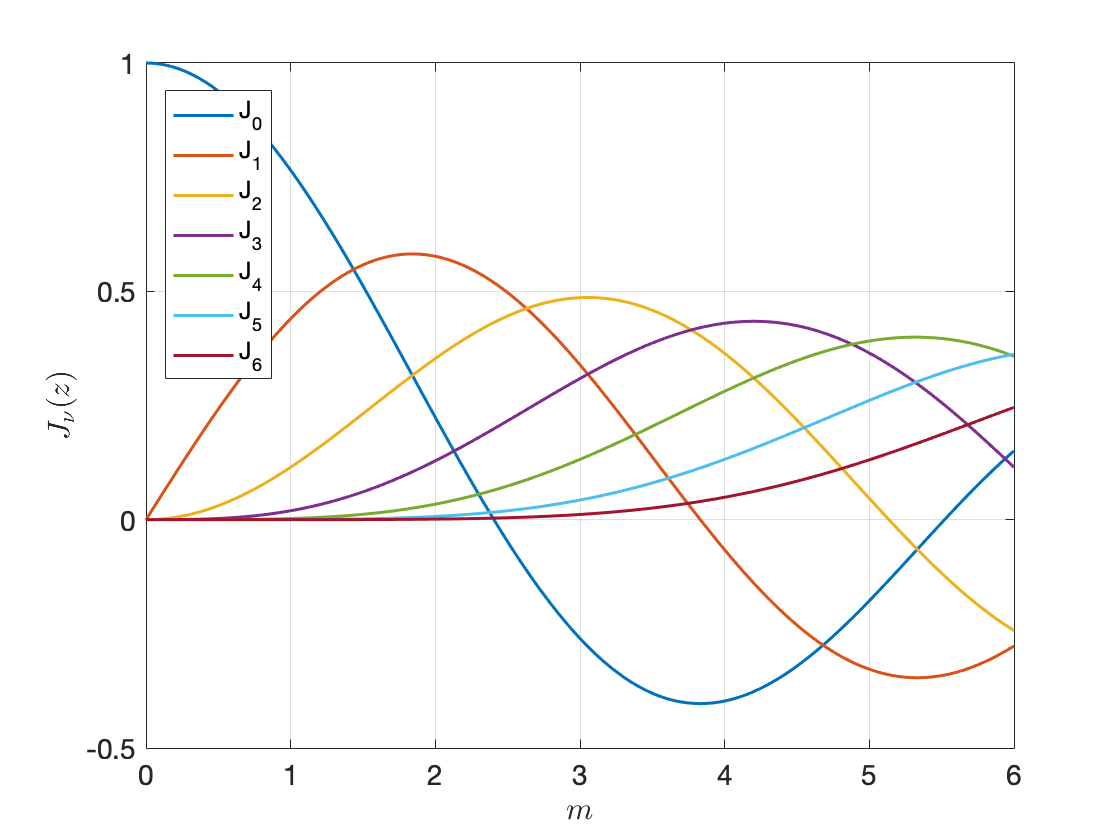
\includegraphics[width=\textwidth]{bessel.png}
		\end{figure}

	\end{column}
	\begin{column}{.48\textwidth}
			\begin{itemize}
			\item $m$ usually small ($\leq 2$)
			\item $J_k (m)$ decrease fast with $k$
			\item Series can be truncated
			\item \textbf{Finite number of frequencies can be coupled}
		\end{itemize}
	\end{column}%
	\hfill
	\end{columns}
	
	\begin{figure}
		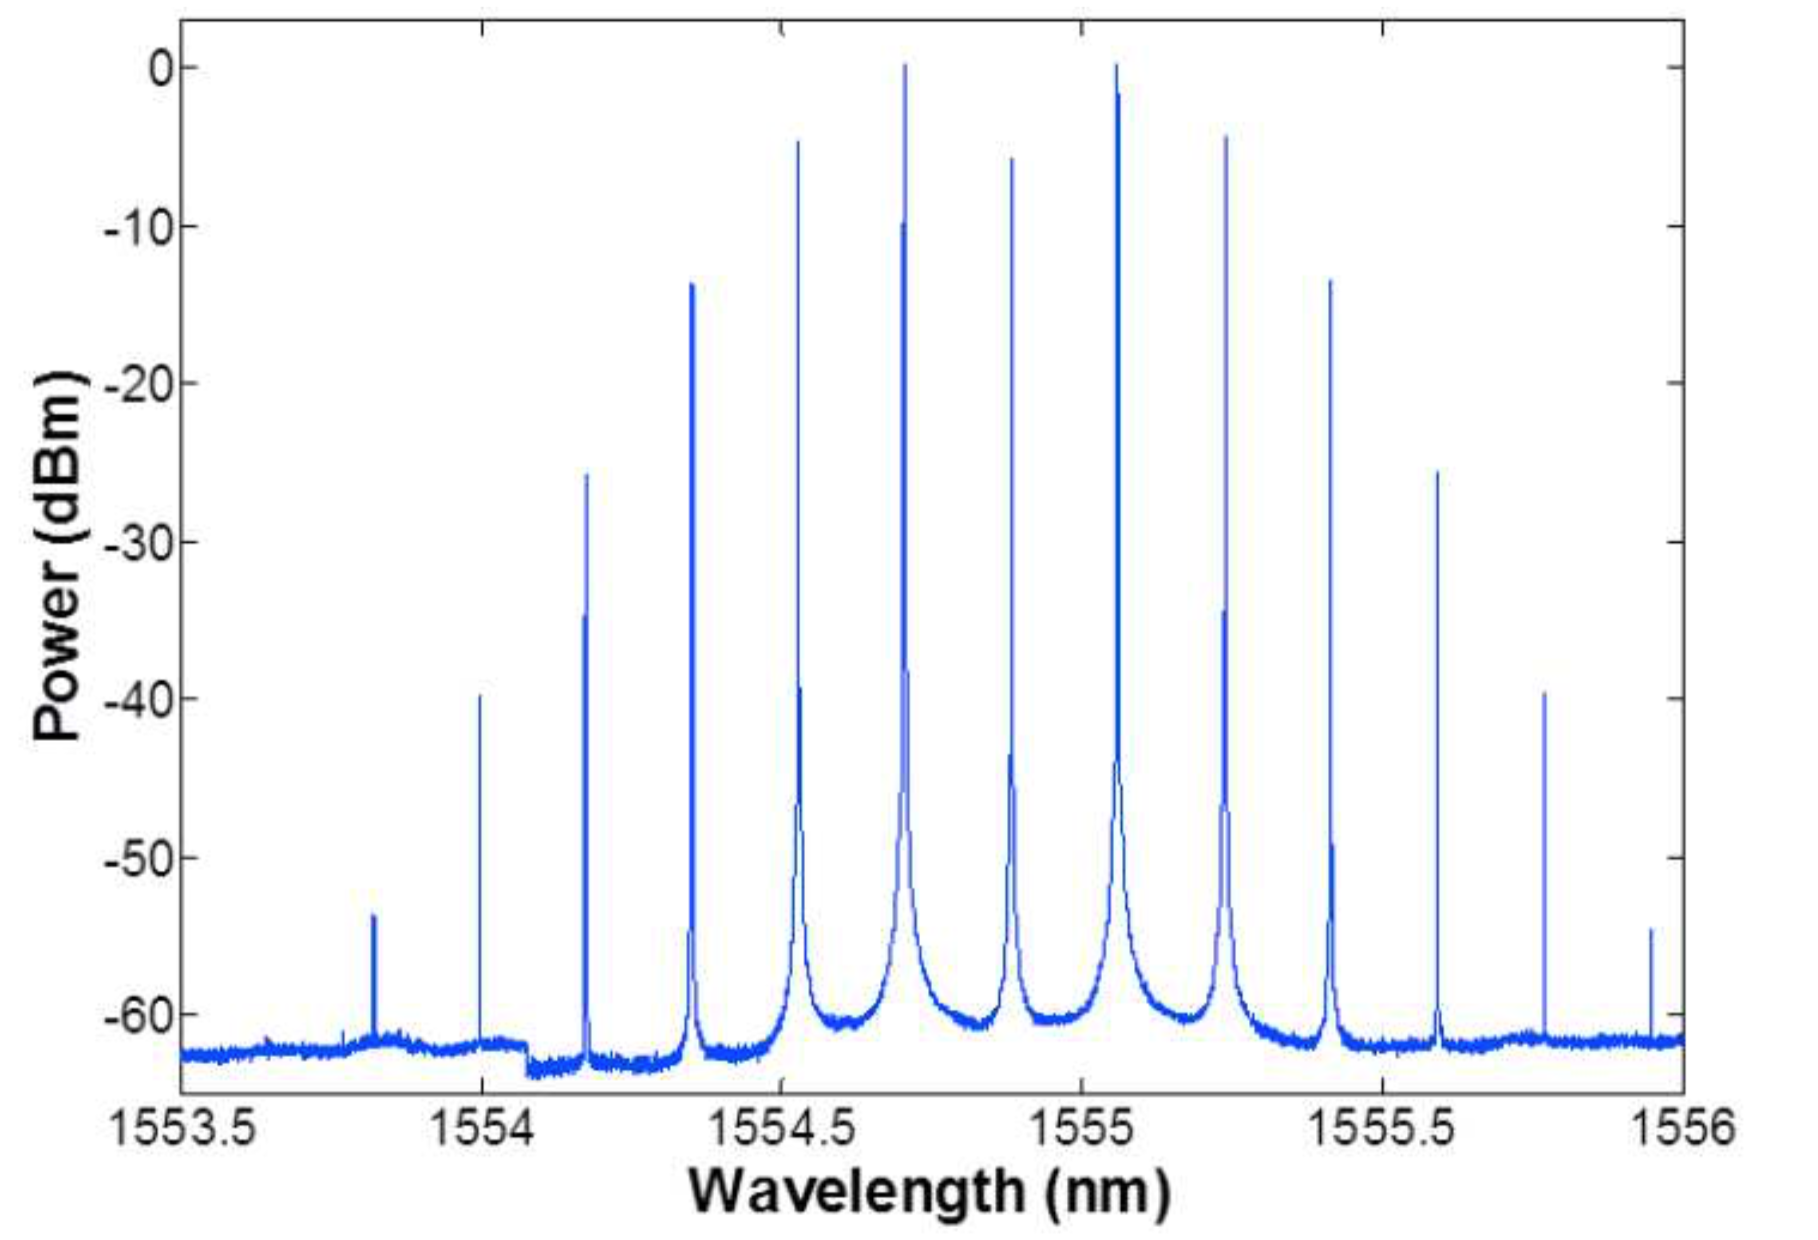
\includegraphics[width=.8\textwidth]{power-in-neurons.png}
		\caption{Spectrum inside the cavity. 13 frequencies are usable.\cite{AkroutAkram2016Pprc}}
	\end{figure}
	
\end{frame}


\begin{frame}
	\begin{figure}
		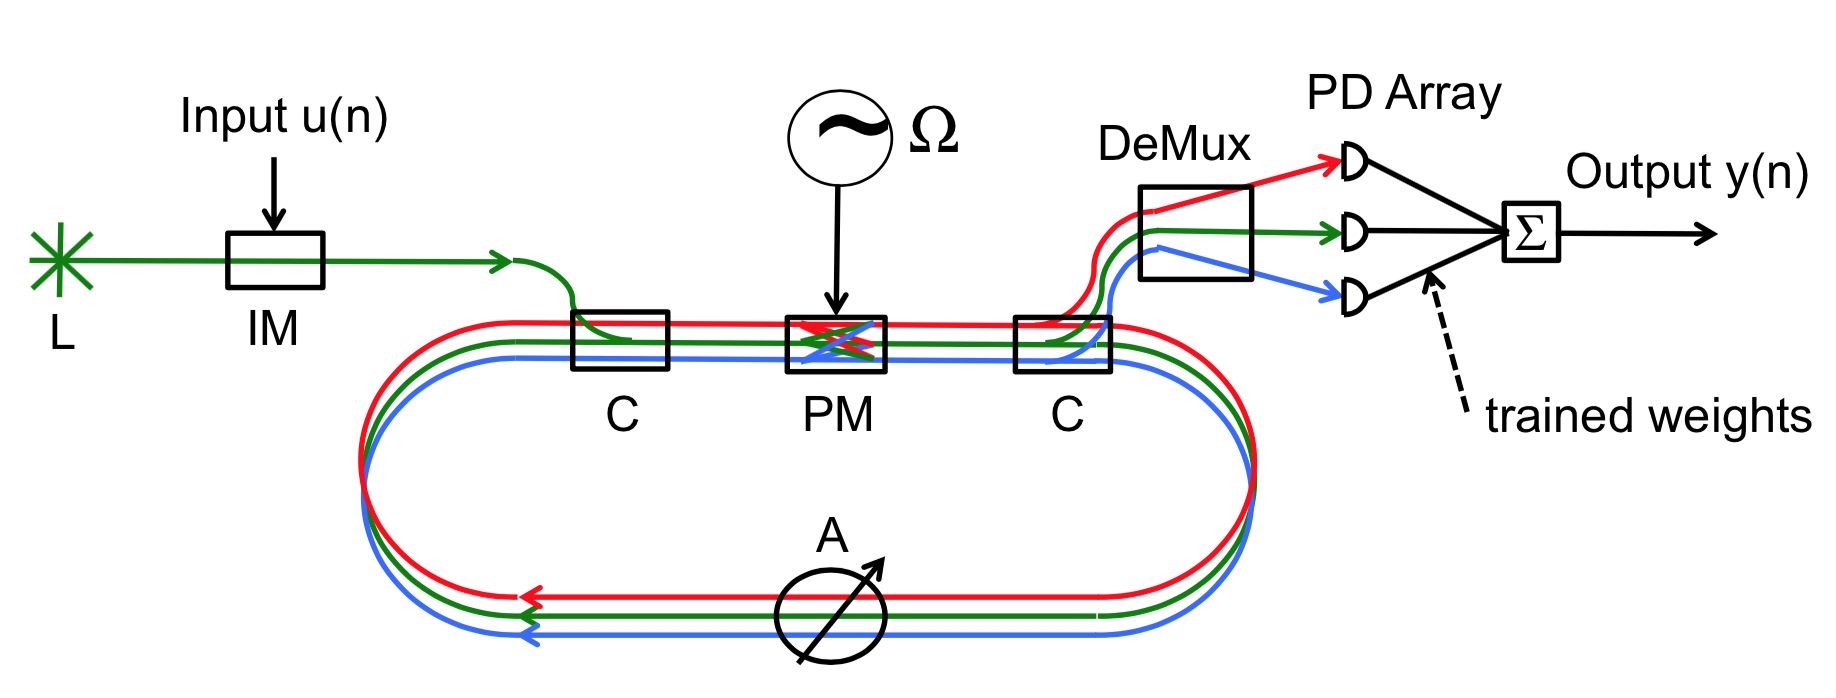
\includegraphics[width=.7\textwidth]{wdm_rc_principle.png}
		\caption{\cite{AkroutAkram2016Pprc}}
	\end{figure}
	
\end{frame}
